\documentclass[10pt,a4paper]{article}
\usepackage[latin1]{inputenc}
\usepackage[english]{babel}
\usepackage{amsmath}
\usepackage{amsfonts}
\usepackage{amssymb}
\usepackage{graphicx}
\usepackage{listings}
\usepackage{wrapfig}
\usepackage{url}

\author{Sascha Wernegger}
\title{Key-Point based Image Retrieval under ISO Still
Image Compression Standards}
 
\begin{document}
\maketitle

\begin{abstract}
In this paper, we examine the influence of JPEG, JPEG-200 and JPEG-XR on local features. Therefore we use the \textbf{VLBenchmarks} \footnote{\url{http://www.vlfeat.org/benchmarks/}} software to calculate the performance of a key point detector using a content based image retrieval system. The data set we used is the \textbf{Oxford Buildings Dataset} \footnote{\url{http://www.robots.ox.ac.uk/~vgg/data/oxbuildings/}};
To compare the influence of compression on the retrieval benchmark, we compress the data set to the different compression formats, and run the benchmark again. We then show the results of our survey.
\end{abstract}

\section{Experiment Setup}
First we will show what software we used to compressed our data, then we will show the used parameters and what compression ratio we achieved. We also discuss the fact that the data set is already compressed in JPEG and what influence it has for the survey.\\
Next we will discuss our setup for the retrieval benchmark, and the results it provides us, so we can compare them. We will also quickly introduce the local feature detectors we tested,and show how we set them up for our experiment.

\subsection{Compression}
To run our experiment we need to compress the Oxford Buildings Dataset to different formats and different compression ratios. Since both the compression, and benchmark duration heavily depends on the size of the data set we decided to use only a subset of 5062 images of the Oxford Buildings Dataset. In the end we got a random subset containing 597 images and reduced the number of queries from 55 to 18.\\
For compression we created a script that doubles the compression ratio until the minimum is reached. Now we want to introduce the different command line tools we used to compress the images and what parameter we used.
Fore JPEG and JPEG-2000 we used the command line tool from \textbf{ImageMagick 7.0.2-5} \footnote{\url{http://www.imagemagick.org/script/index.php}}. We simply used the quality parameter to reduce the filesize.
For details on the usage of the tools we want to refer to the documentation of the tools.\\
Finaly we got 25 data sets: 6 compressed to JPEG, 8 compressed to JPEG-XR, 10 compressed to JPEG-2000 and the original data set. The following figure [\ref{fig:compression}] shows the maximum achieved compression ratio for the different formats.\\
\begin{figure}[!htp]
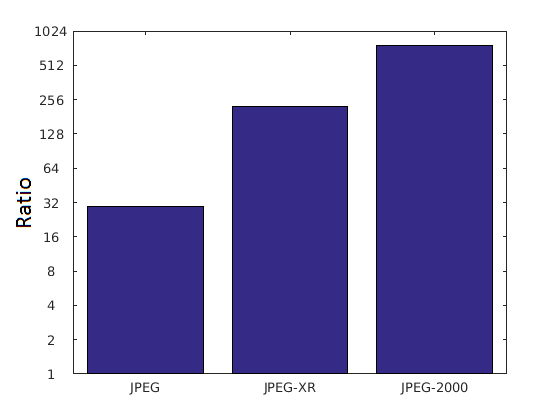
\includegraphics[width=\textwidth]{img/compression.png}
	\caption{Achieved compression ratio for the different formats}
  \label{fig:compression}
\end{figure}
The next thing we discuss is the fact that the Oxford Building Dataset is already compressed in JPEG. For that reason we have calculated the average raw size of the images to compare it with the size of the Oxford Buildings Dataset. The average size as a raw image with 24bpp is about 2,296,754 bytes. The average size of an image from the Oxford Buildings Dataset is 387,864 bytes. So we come up with an initial compression ratio of about 5.92. The following figure [\ref{fig:jpg_ratio}] shows that the quality parameter is set to about 80\% which is introducing only little information loss to the image since everything above 90\% is loss less anyway, and we have much room left to compress our images.
\begin{figure}[!htp]
	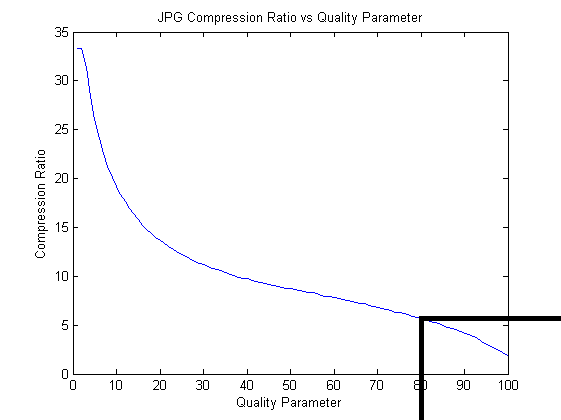
\includegraphics[width=\textwidth]{img/jpg-ratio.png}
	\caption{Estimated Quality Parameter}
  \label{fig:jpg_ratio}
\end{figure}

\subsection{Retrieval Benchmark}
The VLBenchmatk software for Matlab provides a simple to use retrieval benchmark tool. The retrieval benchmark closely follows the work Jegou et. al \cite{inria}. First a set of local features is detected by selected feature extractor and the corresponding  frame is calculated. Next the frame is used to compute descriptor for that frame. To find most similar a K-Nearest neighbours search is used to calculate the descriptor distance. Now the knn-descriptors vote for their image based on their descriptor distances, to finally sort the images.\\
The proposed performance measure for such a retrieval system is the mean average precision(MAP) as described in \cite{philbin}. To calculate the MAP the precision and recall for each document has to be calculated. Since there are four categories in the Oxford Buildings Dataset, we will quickly discuss their meaning
\begin{itemize}
	\item \textbf{Good}  A nice, clear picture of the object/building.
	\item \textbf{OK} More than 25\% of the object is clearly visible. 
	\item \textbf{JUNK} Less than 25\% of the object is visible, or there are very high levels of occlusion or distortion. 
	\item \textbf{BAD} The object is not present. 
\end{itemize}
and usage.
\begin{itemize}
	\item \textbf{Good and OK} Are treated as relevant.
	\item \textbf{JUNK} Is treated as if it is not present in the database
	\item \textbf{BAD} Treated as not relevant.
\end{itemize}
So the query average precision for a query simply is the average of the precision values from each relevant document in the query. And the MAP for all queries is simply the average of the query average precision.

\subsection{Key-Point detectors}
The key-point detectors have two purposes:
\begin{itemize}
	\item Detect key-points
	\item Compute descriptor
\end{itemize}
First the image is searched for key-points, mostly edges,corners or blobs. Next a frame for that key-point  is computed. The frame created can be of different types: point. circle, oriented circle, ellipse, oriented ellipse. Next the feature is computed using the region defined by that frame. The resulting descriptor is stored as a vector of values, for which the distance can be computed. The following sections list the detectors and parameters used.

\subsubsection{Scale Invariant Feature Transform (SIFT)}
SIFT is probably the most well known key-point detector. Since SIFT is included in the VLFeat Software and its parameters seemed to work pretty good we used the default parameters for it which you can look up in the documentation for \textbf{VLFeat} \footnote{\url{http://www.vlfeat.org/matlab/vl_sift.html} }. The VLFeat SIFT implementation only slightly differs from the original implementation of D. Lowe \cite{lowe}. We will shortly discuss the different stages of Sift, but for details we want to refer to \cite{}For key-point detection the Difference of Gaussian is used. Now frames are computed as oriented circles, therefore the orientation is assigned based on the gradient of the image. Finally the descriptor is calculated to generate a histogram of gradients. The resulting vector contains 128 fields.

\subsubsection{Pyramid Histogram Of Visual Words(PHOW)}
The PHOW \cite{phow} features are a variation of dense SIFT descriptors,
extracted at multiple scales. Dense SIFT is a version of SIFT that calculates the descriptors for a window that is sliding across the image. A color version, extracts descriptors
on the three color channels and stacks them up.
When computing descriptors for many keypoints differing only
by their position (and with null rotation), further
simplifcations are possible. To reduce the number of descriptors we changed the \textbf{Step} parameter to 16.

\subsection{Speed Up Robust Features(SURF)}
SURF \cite{surf} is a detector similar to sift, but as the name suggests, it is faster to compute. In SURF, square-shaped Filters are used as an approximation of Gaussian smoothing. for key-point detection a Hessian matrix and Non-maximum is used. Orientation assignment uses a Sliding orientation window using Gaussian weighted Haarwavelet responses from circular neighborhood suppression. The descriptor is calculated using an oriented 4x4 grid that defines sub-region.
Wavelet responses computed for 5x5 samples of the sub-region. For SURF we reduced the treshold  for the keypoint-detection to get more key-points and  increased both the number of octaves int he gaussian pyramid from 4 to 8 and also the number of layers per octave from 2 to 4. For details on the parameters we want to refer to the online documentation of OpenCV \footnote{\url{http://docs.opencv.org/2.4/modules/nonfree/doc/feature_detection.html}}.

\subsection{Oriented FAST and Rotated Brief (ORB)}
ORB \cite{orb} uses FAST \cite{fast1} \cite{fast2} to detect corners as key-points. The orientation is calculated using the centroid operator. Dimensionality reduction for the descriptors can be achieved by using hash functions that reduce SIFT descriptors to binary strings. The fast key-point detection and small descriptor size makes it well suited for devices with limited resources. The orb detector lets you specify the number of key-points, to limit the number of detected key-points. We decided to use as much descriptors as possible, setting the number of features to 8000 which is about three times the number of features created from the other descriptors, compensating the descriptor size. We also changed the scale factor from 1.2 to 1.1 and increased the number of scale levels to 16 to get more key-points.For details on the parameters we want to refer to the online documentation of OpenCV \footnote{\url{http://docs.opencv.org/2.4/modules/nonfree/doc/feature_detection.html}}.

\section{Results}

First we want to show the MAP for the original data set shown in fig. \ref{fig:map}.
In the next sections we will see how the detectors have performed. Therefore we show plots of the MAP over the compression ratio.

\begin{figure}[!htp]
	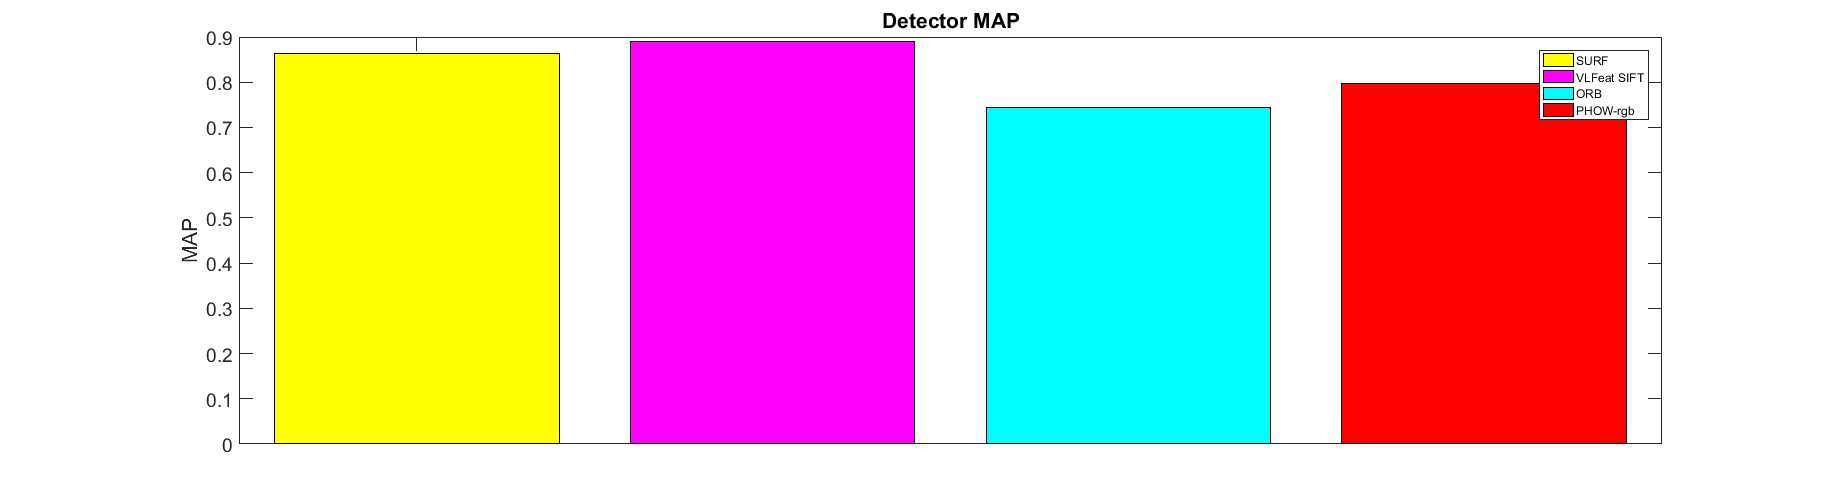
\includegraphics[width=1.2\textwidth]{img/refmap.png}
	\caption{MAP for the different descriptors on the original data set}
	\label{fig:map}
\end{figure}

For the interpretation of the results we also calculated the Mean Peak Signal to Noise Ratio (PSNR) fig. \ref{fig:psnr} for the compressed data sets, to see if there is some relation to the noise contribution.
\begin{figure}[!htp]
	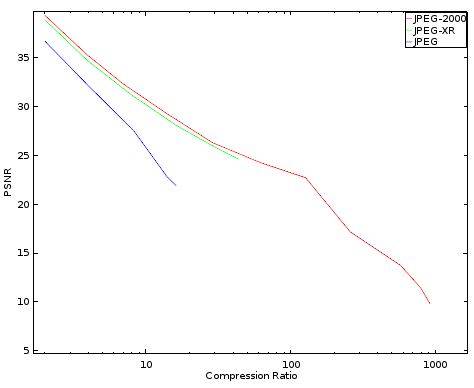
\includegraphics[width=\textwidth]{img/psnr.png}
	\caption{This shows the mean-PSNR calculated for the different compressed data
	\label{fig:psnr} sets}
\end{figure} 

\begin{figure}[!htp]
	\begin{tabular}{|c|}
		\hline \\
		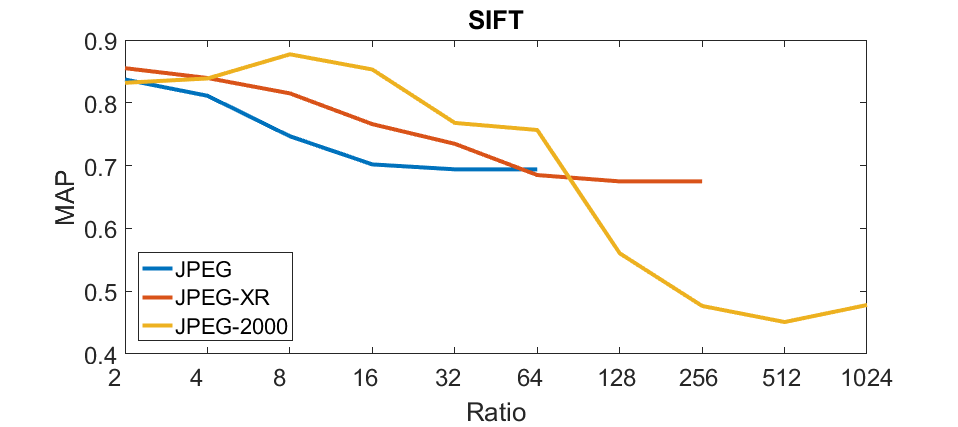
\includegraphics[width = \textwidth]{img/sift_map.png}\\
		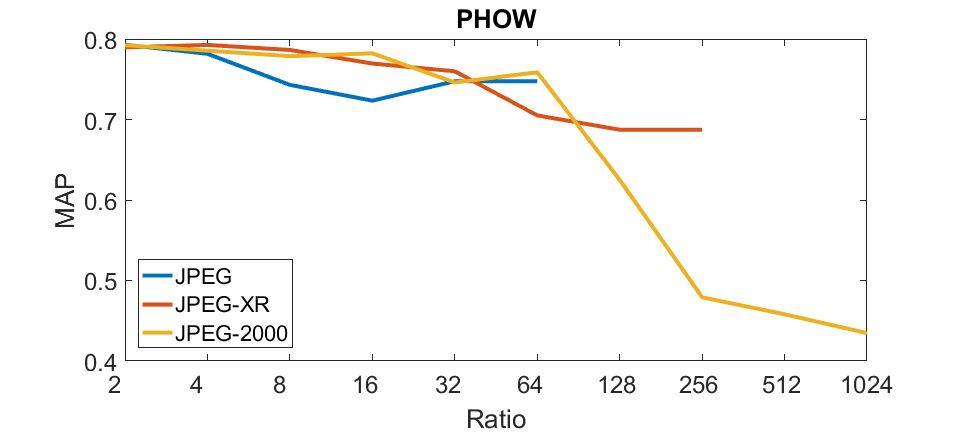
\includegraphics[width = \textwidth]{img/phow_map.png}\\
		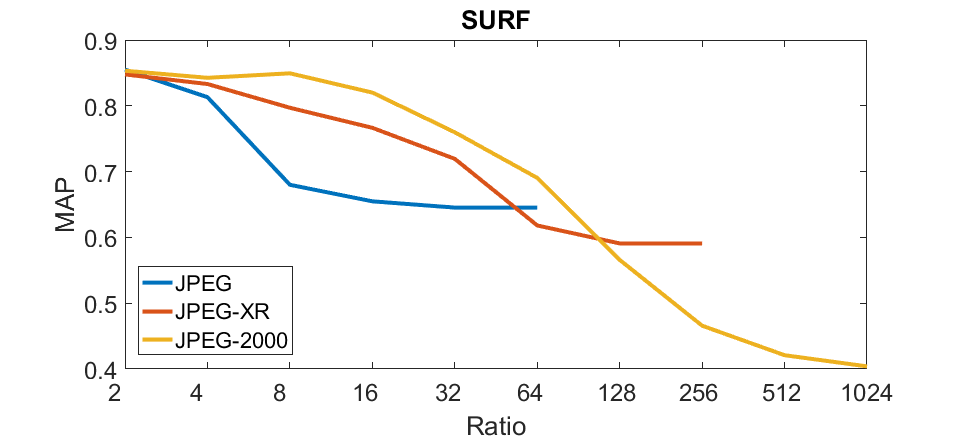
\includegraphics[width = \textwidth]{img/surf_map.png}\\
		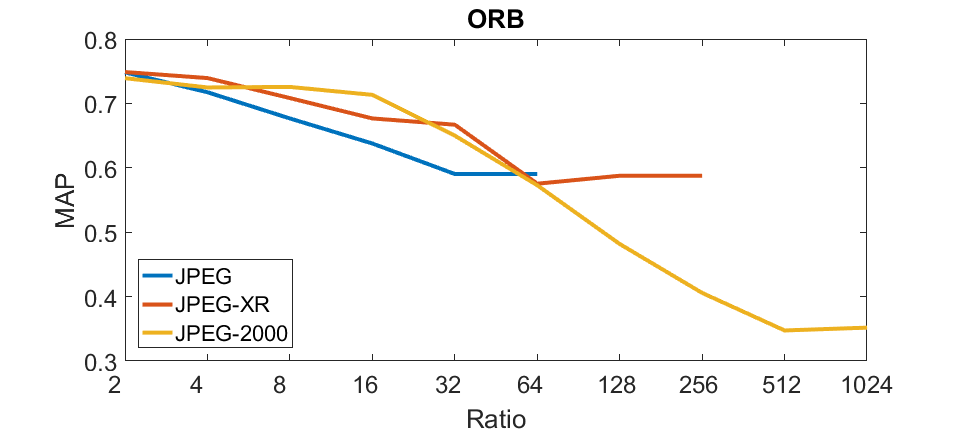
\includegraphics[width = \textwidth]{img/orb_map.png}\\
		\hline
	\end{tabular}
	\caption{plot of MAP over compression ratio for the different
	\label{fig:maps} detectors and formats}
\end{figure}


\newpage
\bibliographystyle{plain}
\bibliography{paper} 

\end{document}